\documentclass{book}

\usepackage{amsmath}
\usepackage{alltt}
\usepackage{amssymb}
\usepackage{chemfig}
\usepackage{mathtools}
\usepackage{listings}
\usepackage{wrapfig}
\usepackage{color}
\usepackage{float}
\usepackage{caption}
\usepackage{subcaption}
\usepackage{mhchem}
\usepackage{multicol}
\usepackage{paralist}
\usepackage{tcolorbox}
\usepackage{braket}
\usepackage[framemethod=TikZ]{mdframed}
\usepackage[english]{babel}
\usepackage[utf8x]{inputenc}
\usepackage[colorinlistoftodos]{todonotes}
\usepackage{esint}
\usepackage{hyperref}
\hypersetup{
    colorlinks=true,
    linkcolor=blue,
    filecolor=magenta,      
    urlcolor=cyan,
}

\def\msquare{\mathord{\scalebox{1.5}[1]{\scalerel*{\Box}{\strut}}}}

\title{Research Notes}
\date{2020-04-05}
\author{Kalp Shah}

\lstdefinestyle{shared}{
    belowcaptionskip=1\baselineskip,
    breaklines=true,
    xleftmargin=\parindent,
    showstringspaces=false,
    basicstyle=\fontsize{10}{6}\ttfamily,
}
\lstdefinestyle{cpp}{
	style=shared,
    language=C++,
    keywordstyle=\bfseries\color{green!40!black},
    commentstyle=\itshape\color{red!80!black},
    identifierstyle=\color{blue},
    stringstyle=\color{purple!40!black},
}
\lstdefinestyle{java}{
    style=shared,
    language=Java,
    keywordstyle=\bfseries\color{green!40!black},
    commentstyle=\itshape\color{purple!40!black},
    identifierstyle=\color{blue},
    stringstyle=\color{orange},
}
\lstdefinestyle{py}{
    style=shared,
    language=Python,
    keywordstyle=\bfseries\color{green!40!black},
    commentstyle=\itshape\color{purple!40!black},
    identifierstyle=\color{blue},
    stringstyle=\color{orange},
}
\lstdefinestyle{txt}{
    style=shared,
}
\lstset{escapechar=@}

\newcounter{theo}[section]\setcounter{theo}{0}
\renewcommand{\thetheo}{\arabic{section}.\arabic{theo}}
\newenvironment{theorem}[2][]{%
\refstepcounter{theo}%
\ifstrempty{#1}%
{\mdfsetup{%
frametitle={%
\tikz[baseline=(current bounding box.east),outer sep=0pt]
\node[anchor=east,rectangle,fill=blue!20]
{\strut Theorem~\thetheo};}}
}%
{\mdfsetup{%
frametitle={%
\tikz[baseline=(current bounding box.east),outer sep=0pt]
\node[anchor=east,rectangle,fill=blue!20]
{\strut Theorem~\thetheo:~#1};}}%
}%
\mdfsetup{innertopmargin=10pt,linecolor=blue!20,%
linewidth=2pt,topline=true,%
frametitleaboveskip=\dimexpr-\ht\strutbox\relax
}
\begin{mdframed}[]\relax%
\label{#2}}{\end{mdframed}}


\newcounter{prf}[section]\setcounter{prf}{0}
\renewcommand{\theprf}{\arabic{section}.\arabic{prf}}
\newenvironment{proof}[2][]{%
\refstepcounter{prf}%
\ifstrempty{#1}%
{\mdfsetup{%
frametitle={%
\tikz[baseline=(current bounding box.east),outer sep=0pt]
\node[anchor=east,rectangle,fill=red!20]
{\strut Proof~\theprf};}}
}%
{\mdfsetup{%
frametitle={%
\tikz[baseline=(current bounding box.east),outer sep=0pt]
\node[anchor=east,rectangle,fill=red!20]
{\strut Proof~\thetheo:~#1};}}%
}%
\mdfsetup{innertopmargin=10pt,linecolor=red!20,%
linewidth=2pt,topline=true,%
frametitleaboveskip=\dimexpr-\ht\strutbox\relax
}
\begin{mdframed}[]\relax%
\label{#2}}{\end{mdframed}}


\newcounter{prob}[section]\setcounter{prob}{0}
\renewcommand{\theprob}{\arabic{section}.\arabic{prob}}
\newenvironment{problem}[2][]{%
\refstepcounter{prob}%
\ifstrempty{#1}%
{\mdfsetup{%
frametitle={%
\tikz[baseline=(current bounding box.east),outer sep=0pt]
\node[anchor=east,rectangle,fill=red!60]
{\strut Problem~\theprob};}}
}%
{\mdfsetup{%
frametitle={%
\tikz[baseline=(current bounding box.east),outer sep=0pt]
\node[anchor=east,rectangle,fill=red!60]
{\strut Problem~\theprob:~#1};}}%
}%
\mdfsetup{innertopmargin=10pt,linecolor=red!60,%
linewidth=2pt,topline=true,%
frametitleaboveskip=\dimexpr-\ht\strutbox\relax
}
\begin{mdframed}[]\relax%
\label{#2}}{\end{mdframed}}


\newcounter{exm}[section]\setcounter{exm}{0}
\renewcommand{\theexm}{\arabic{section}.\arabic{exm}}
\newenvironment{example}[2][]{%
\refstepcounter{exm}%
\ifstrempty{#1}%
{\mdfsetup{%
frametitle={%
\tikz[baseline=(current bounding box.east),outer sep=0pt]
\node[anchor=east,rectangle,fill=green!20]
{\strut Example~\theexm};}}
}%
{\mdfsetup{%
frametitle={%
\tikz[baseline=(current bounding box.east),outer sep=0pt]
\node[anchor=east,rectangle,fill=green!20]
{\strut Example~\thetheo:~#1};}}%
}%
\mdfsetup{innertopmargin=10pt,linecolor=green!20,%
linewidth=2pt,topline=true,%
frametitleaboveskip=\dimexpr-\ht\strutbox\relax
}
\begin{mdframed}[]\relax%
\label{#2}}{\end{mdframed}}


\newcounter{def}[section]\setcounter{def}{0}
\renewcommand{\thedef}{\arabic{section}.\arabic{def}}
\newenvironment{definition}[2][]{%
\refstepcounter{def}%
\ifstrempty{#1}%
{\mdfsetup{%
frametitle={%
\tikz[baseline=(current bounding box.east),outer sep=0pt]
\node[anchor=east,rectangle,fill=purple!20]
{\strut Definition~\thedef};}}
}%
{\mdfsetup{%
frametitle={%
\tikz[baseline=(current bounding box.east),outer sep=0pt]
\node[anchor=east,rectangle,fill=purple!20]
{\strut Definition~\thetheo:~#1};}}%
}%
\mdfsetup{innertopmargin=10pt,linecolor=purple!20,%
linewidth=2pt,topline=true,%
frametitleaboveskip=\dimexpr-\ht\strutbox\relax
}
\begin{mdframed}[]\relax%
\label{#2}}{\end{mdframed}}

\newcounter{note}[section]\setcounter{note}{0}
\renewcommand{\thenote}{\arabic{section}.\arabic{note}}
\newenvironment{note}[2][]{%
\refstepcounter{note}%
\ifstrempty{#1}%
{\mdfsetup{%
frametitle={%
\tikz[baseline=(current bounding box.east),outer sep=0pt]
\node[anchor=east,rectangle,fill=yellow!40!green!50]
{\strut Note~\thenote};}}
}%
{\mdfsetup{%
frametitle={%
\tikz[baseline=(current bounding box.east),outer sep=0pt]
\node[anchor=east,rectangle,fill=yellow!40!green!50]
{\strut Note~\thenote:~#1};}}%
}%
\mdfsetup{innertopmargin=10pt,linecolor=yellow!40!green!50,%
linewidth=2pt,topline=true,%
frametitleaboveskip=\dimexpr-\ht\strutbox\relax
}
\begin{mdframed}[]\relax%
\label{#2}}{\end{mdframed}}

\newcounter{lem}[section]\setcounter{lem}{0}
\renewcommand{\thelem}{\arabic{section}.\arabic{lem}}
\newenvironment{lemma}[2][]{%
\refstepcounter{lem}%
\ifstrempty{#1}%
{\mdfsetup{%
frametitle={%
\tikz[baseline=(current bounding box.east),outer sep=0pt]
\node[anchor=east,rectangle,fill=teal!20]
{\strut Lemma~\thelem};}}
}%
{\mdfsetup{%
frametitle={%
\tikz[baseline=(current bounding box.east),outer sep=0pt]
\node[anchor=east,rectangle,fill=teal!20]
{\strut Definition~\thelemm:~#1};}}%
}%
\mdfsetup{innertopmargin=10pt,linecolor=teal!20,%
linewidth=2pt,topline=true,%
frametitleaboveskip=\dimexpr-\ht\strutbox\relax
}
\begin{mdframed}[]\relax%
\label{#2}}{\end{mdframed}}


\let\cleardoublepage\clearpage


\begin{document}
\pagenumbering{arabic}


\begin{titlepage}
    \newcommand{\HRule}{\rule{\linewidth}{0.5mm}}
    \center
    \textsc{\LARGE International Institute of Information Technology, Hyderabad}\\[0.5cm]
    
\includegraphics[scale=1]{img/iiit-logo.jpeg}\\[0.5cm]
    \textsc{\Large Systems Biology}\\[0.5cm]
    \textsc{\large Adaptation Mechanisms in Phosphorylation Cycles}\\[0.5cm] % Minor heading such as course title
    \HRule \\[0.4cm]
    { \huge \bfseries Project Notes}\\[0.4cm]
    \HRule \\[1.5cm]
    \begin{minipage}{0.6\textwidth}
    \begin{flushleft} \large
    \emph{Author:} Kalp Shah
    \end{flushleft}
    \end{minipage}\\[2cm]
    {\large \today}\\[2cm]
    \vfill
\end{titlepage}

\chapter{Introduction}

\chapter*{Mass Action Results}

This chapter contains all the analysis done 
in the original paper and the conclusions that 
it came up with. This is very similar to the original 
paper itself but is redone again to make the compare 
and contrast easier to understand and make the steps 
followed easier to understand.

\section*{System Description}
The following phosphorylation system is used for studying :

\begin{center}
    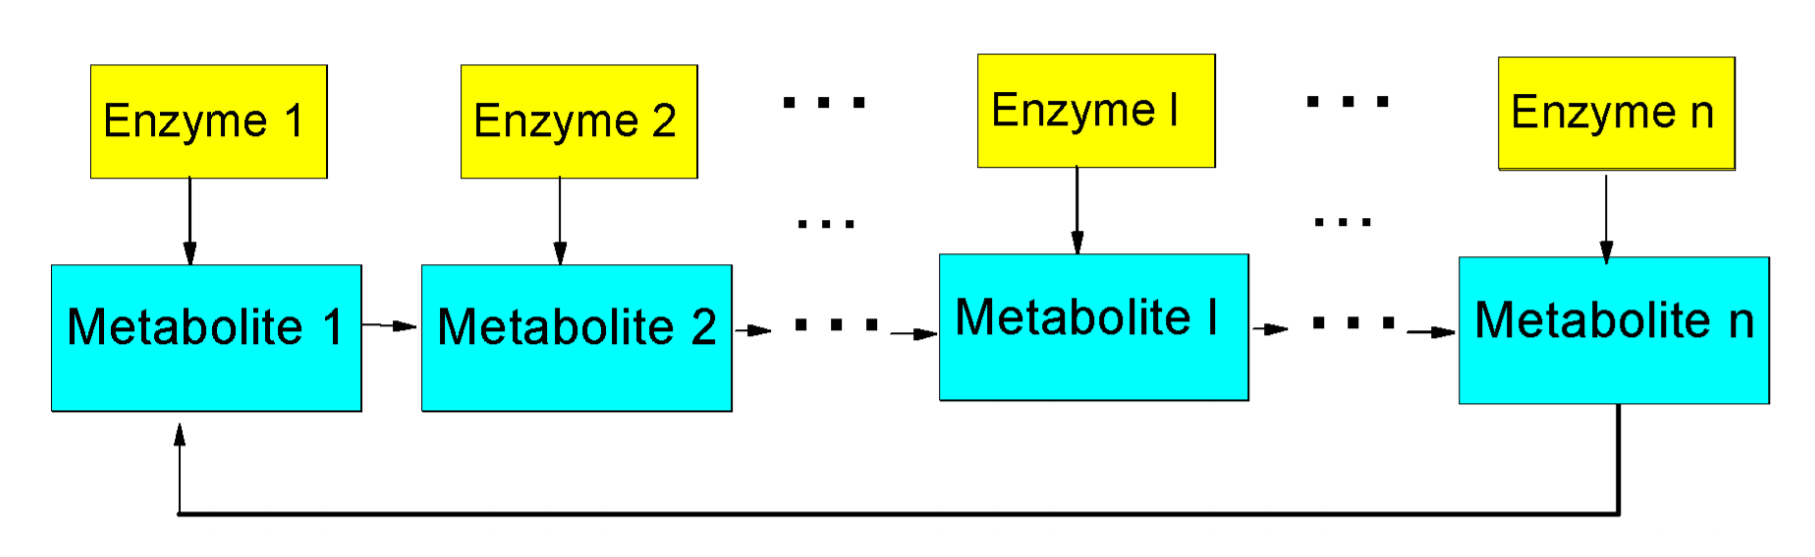
\includegraphics[scale=0.3]{img/orig-sys.png}
\end{center}

\subsection*{Rate Equations}
\noindent This corresponds to the following set of reactions :

$$ \ce{X_i + E_i <=>[K_{i,1}][K_i,2] X_iE_i -> X_{i+1} + E_i}$$

\noindent Which then corresponds to the following rate equations :

\begin{align*}
    \frac{d[X_i]}{dt} &= -K_{i,1}[X_i][E_i] + K_{i,2}[X_iE_i] + K_{i-1,3}[X_{i-1}E_{i-1}]\\
    \frac{d[E_i]}{dt} &= -K_{i,1}[X_i][E_i] + (K_{i,2} + K_{i,3})[X_iE_i]\\
    \frac{d[X_iE_i]}{dt} &= K_{i,1}[X_i][E_i] - (K_{i,2} + K_{i,3})[X_iE_i]
\end{align*}

\noindent As the amount of enzyme remains constant in the 
system, the equations can be rewritten as follows :

\begin{align*}
    \frac{d[X_i]}{dt} &= K_{i,1}[X_i][X_iE_i] + K_{i,2}[X_iE_i] + K_{i-1,3}[X_{i-1}E_{i-1}] - K_{i,1}[X_i][E_i]_0\\
    \frac{d[E_i]}{dt} &= -K_{i,1}[X_i][X_iE_i] + (K_{i,2} + K_{i,3})[X_iE_i] + K_{i,1}[X_i][E_i]_0 \\
    \frac{d[X_iE_i]}{dt} &= -K_{i,1}[X_i][X_iE_i] - (K_{i,2} + K_{i,3})[X_iE_i] + K_{i,1}[X_i][E_i]_0
\end{align*}

\noindent This is due to the fact that $[E_i]_0 = [E]_i + 
[X_iE_i]$, which can be used to eliminate the $[E_i]$ term 
from the equations. 

\subsection*{Allosteric Binding and Negative Autoregulation}
The paper then goes on to describe the phosphorylation 
cycle with allosteric binding and negative autoregulation. 
The reaction taken to exhibit this phenomenon is the
$\ce{DNA -> mRNA -> Proteins}$, where negative 
autoregulation is described.
\\\\
The paper assumes that autoregulation is done by a reversible 
binding/releasing of free and bound promoters, which is 
described below.

$$ \ce{FP + E_{1total} <=>[K_{allo}][K_{rel}] BP} $$

\noindent In this $FP$ is the free promoter and $BP$ is the 
bound one. The assumption that number of binding sites on 
promoters is very small as compared to concentration of 
proteins, to neglect the effect of binding/releasing 
reaction on the dynamics of the enzyme, is also made.
\\\\
The state equations for these reactions are as follows :

\begin{align*}
    \frac{d[FP]}{dt} &= K_{rel}([FP]_{max} - [FP])\\
    \frac{d[mRNA]}{dt} &= K_{pro}[FP] - K_d[mRNA]\\
    \frac{d[E1]_{total}}{dt} &= K_{tran}[mRNA] - K_{allo}\frac{[X_l][E_1]_{total}}{K_{half} + [E_1]_{total}}
\end{align*}
\newpage
\noindent These equations are for the following reaction :

\begin{center}
    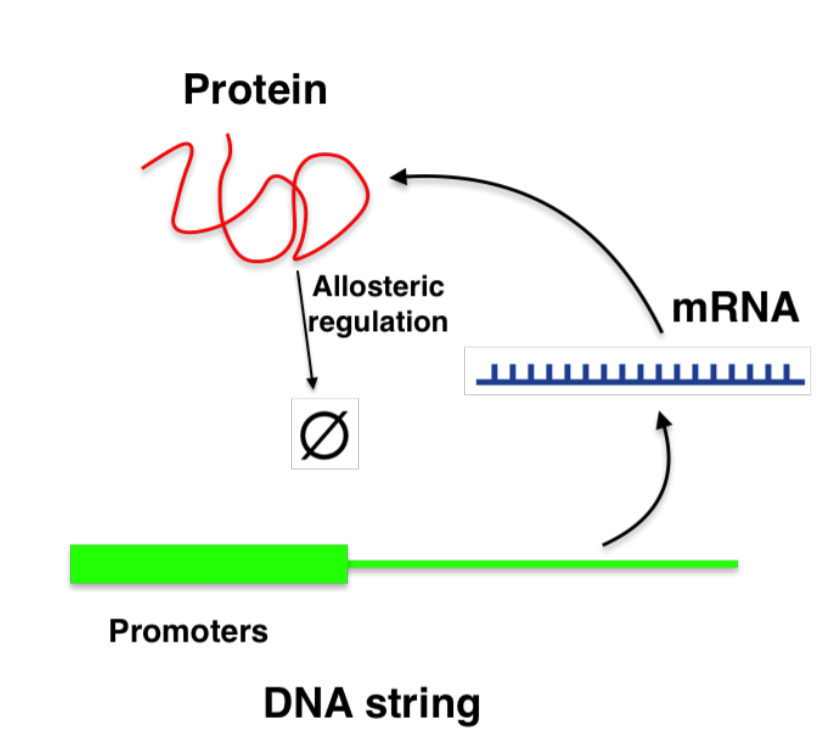
\includegraphics[scale=0.4]{img/dna-noneg.png}
\end{center}

\noindent Another mechanism with negative autoregulation is 
also described by the paper, which is given as follows :

\begin{center}
    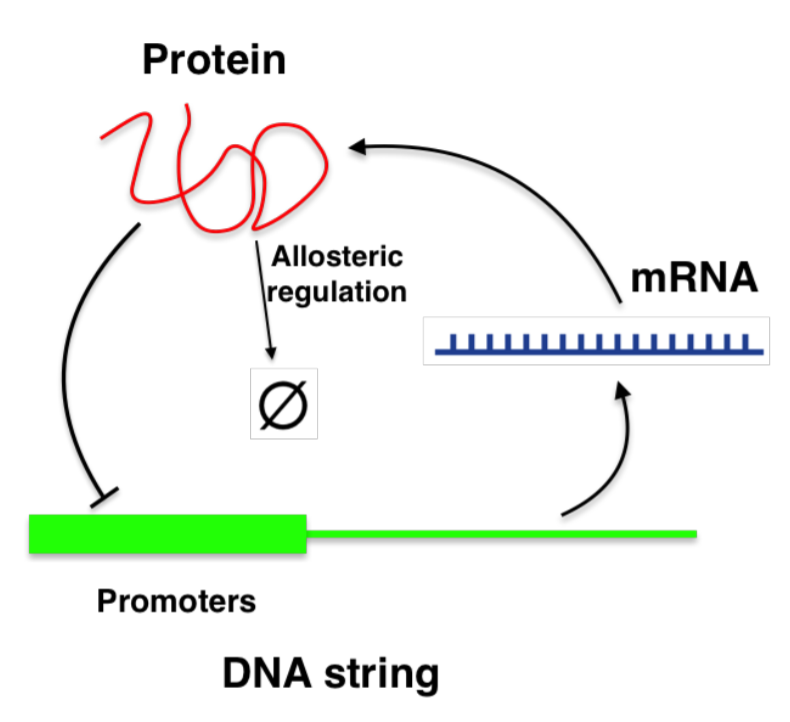
\includegraphics[scale=0.4]{img/dna-neg.png}
\end{center}

\noindent This system is described by the following equations :
\begin{align*}
    \frac{d[FP]}{dt} &= K_{rel}([FP]_{max} - [FP]) - K_{auto}[E_1]_{total}[FP]\\
    \frac{d[mRNA]}{dt} &= K_{pro}[FP] - K_d[mRNA]\\
    \frac{d[E1]_{total}}{dt} &= K_{tran}[mRNA] - K_{allo}\frac{[X_l][E_1]_{total}}{K_{half} + [E_1]_{total}}
\end{align*}

\noindent In these, $[FP]_{max}$ is the total concentration of 
all the promoters. 
\newpage
The reaction with all the rate constants is given as below :

\begin{center}
    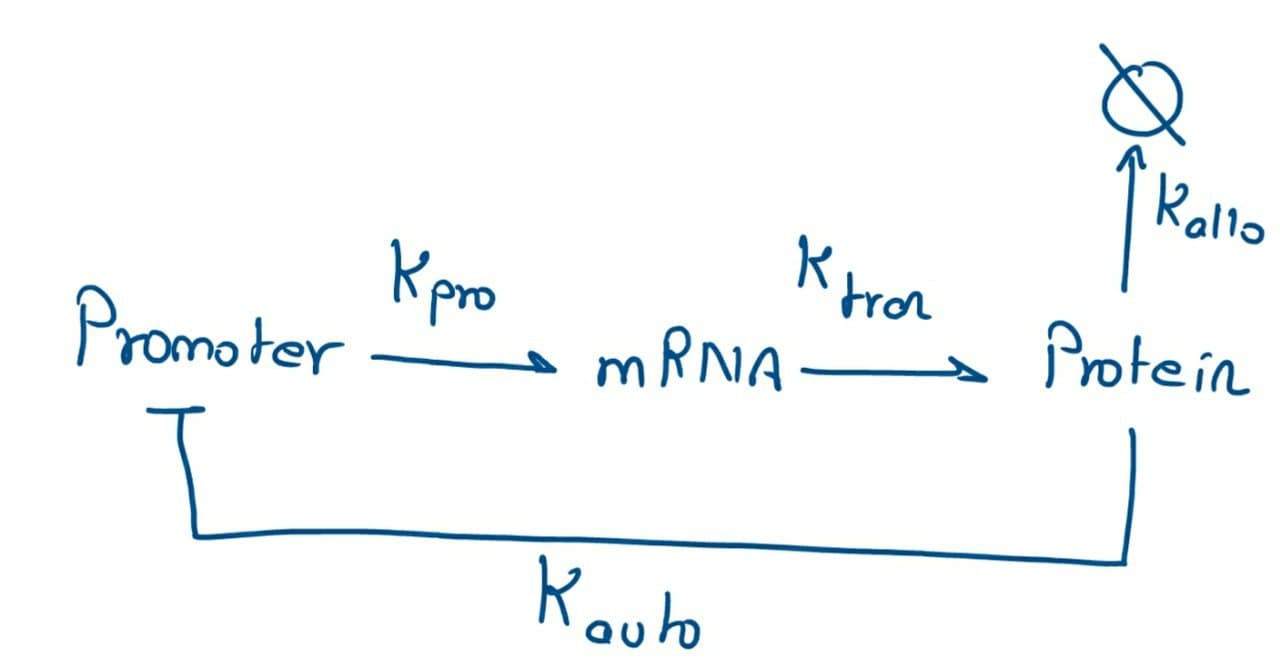
\includegraphics[scale=0.3]{img/eqn-rate.jpg}
\end{center}

\noindent The other constants are as follows :
\begin{itemize}
    \item $K_{\text{half}}$ \\ \indent Concentration of $[E_1]_{total}$ when reaction rate is half-maximum.
    \item $[FP] + [BP] = [FP]_{\text{max}}$
\end{itemize}

\subsection*{Closed Loop Systems}
Thus using the math done above, the rate equations are 
as follows :

\subsubsection*{DNA Cycle}
\begin{align*}
    \frac{d[FP]}{dt} &= K_{rel}([FP]_{max} - [FP]) - K_{auto}[E_1]_{total}[FP]\\
    \frac{d[mRNA]}{dt} &= K_{pro}[FP] - K_d[mRNA]\\
    \frac{d[E1]_{total}}{dt} &= K_{tran}[mRNA] - K_{allo}\frac{[X_l][E_1]_{total}}{K_{half} + [E_1]_{total}}
\end{align*}

\subsubsection*{Phosphorylation Cycle}
\begin{align*}
    \frac{d[X_i]}{dt} &= K_{i,1}[X_i][X_iE_i] + K_{i,2}[X_iE_i] + K_{i-1,3}[X_{i-1}E_{i-1}] - K_{i,1}[X_i][E_i]_0\\
    \frac{d[X_iE_i]}{dt} &= -K_{i,1}[X_i][X_iE_i] - (K_{i,2} + K_{i,3})[X_iE_i] + K_{i,1}[X_i][E_i]_0
\end{align*}

\subsection*{Conclusion}
In the above section, the system was properly defined and in 
the next section, various analysis will be done.

\section*{Analysis}
This is analysis which is done under equilibrium and various 
aspects such as robustness will be analysed.
\subsection*{Robustness}
The robustness of $X_l$ species is checked under both the 
metabolism regulation mechanisms as discussed before. Robustness 
can be examined by using the elasticity metric.
\\\\
A $[S]^*$ is defined, which is the concentration of given 
species $S$ at equilibrium.

\subsubsection{Elasticity Coefficient}
Elasticity Coefficient ($\varepsilon$) is defined as :

$$ \varepsilon = \frac{d \ln{[X_l]^*}}{d \ln[E_1]^*_{\text{total}}}$$

\noindent Thus, the closer $\varepsilon$ is to 0, the more 
robust the system is, as it will try to remain at equilibrium.

\subsubsection*{Derevation}
The deravative of the latent state variable 
$[FP] + \frac{K_{rel}}{K_{pro}}[mRNA] + \frac{K_dK_{rel}}{K_{tran}K_{pro}}[E_1]_{total}$ 
is as follows :

\begin{align*}
    &\frac{d}{dt} ([FP] + \frac{K_{rel}}{K_{pro}}[mRNA] + \frac{K_dK_{rel}}{K_{tran}K_{pro}}[E_1]_{total})\\
    =&-\frac{K_dK{rel}K_{allo}}{K_{tran}K_{pro}} \frac{[X_l][E_1]_{total}}{K_{half}+[E_1]_{total}} + K_{rel}[FP]_{max} - K_{auto}[E_1]_{total}[FP]\\
    =&-K_{gain}([X_l] - R - \frac{K_{half}[X_l]}{K_{half} + [E_1]_{total}} + \frac{K_{auto}}{K_{gain}}[E_1]_{total}[FP])
\end{align*}

\noindent In this, the defined constants are :
\begin{itemize}
    \item $K_{gain} = \frac{K_dK_{rel}K_{allo}}{K_{tran}K_{pro}}$
    \item $R = \frac{K_{rel}[FP]_{max}}{K_{gain}}$
\end{itemize}

\noindent Thus, at equilibrium

\begin{align*}
    [X_l]^* &= (R - \frac{K_{auto}}{K_{gain}}[E_1]^*_{total}[FP]^*)\frac{K_{half}+[E_1]^*_{total}}{[E_1]^*_{total}}\\
    &= R(\frac{K_{rel}}{K_{auto}[E_1]^*_{total} + K_{rel}})\frac{K_{half}+[E_1]^*_{total}}{[E_1]^*_{total}}
\end{align*}

\noindent Thus, elasticity coefficient is :

\begin{equation*}
    \varepsilon = -\frac{K_{auto}[E_1]^*_{total}}{K_{auto}[E_1]^*_{total} + K_{rel}} + \frac{K_{half}}{K_{half} + [E_1]^*_{total}}
\end{equation*}

\subsection*{Conclusion}
Thus, it can be seen that two scenarios occur, which are as 
follows :

\begin{itemize}
    \item $\varepsilon \approxeq 0$\\ \indent $K_{half} \ll [E_1]^*_{total} \ll \frac{K_{rel}}{K_{auto}}$
    \item $\varepsilon \approxeq -1$\\ \indent $[E_1]^*_{total} \gg \max(K_{rel}/K_{auto},K_{half})$ \\ \indent $[E_1]^*_{total} \ll \min(K_{rel}/K_{auto},K_{half})$
\end{itemize}

\noindent This suggests that regulator is highly robust at 
medium levels of $[E_1]^*_{total}$ and fragile at extreme levels 
of it.
\chapter*{Michaelis-Menten Results}
In this section, Michaelis-Menten kinetics is applied to 
the system and the results are compared with the original 
results given in the original paper.

\section*{System Description}
The system reaction is given below, which is same as the one 
given above :

\begin{center}
    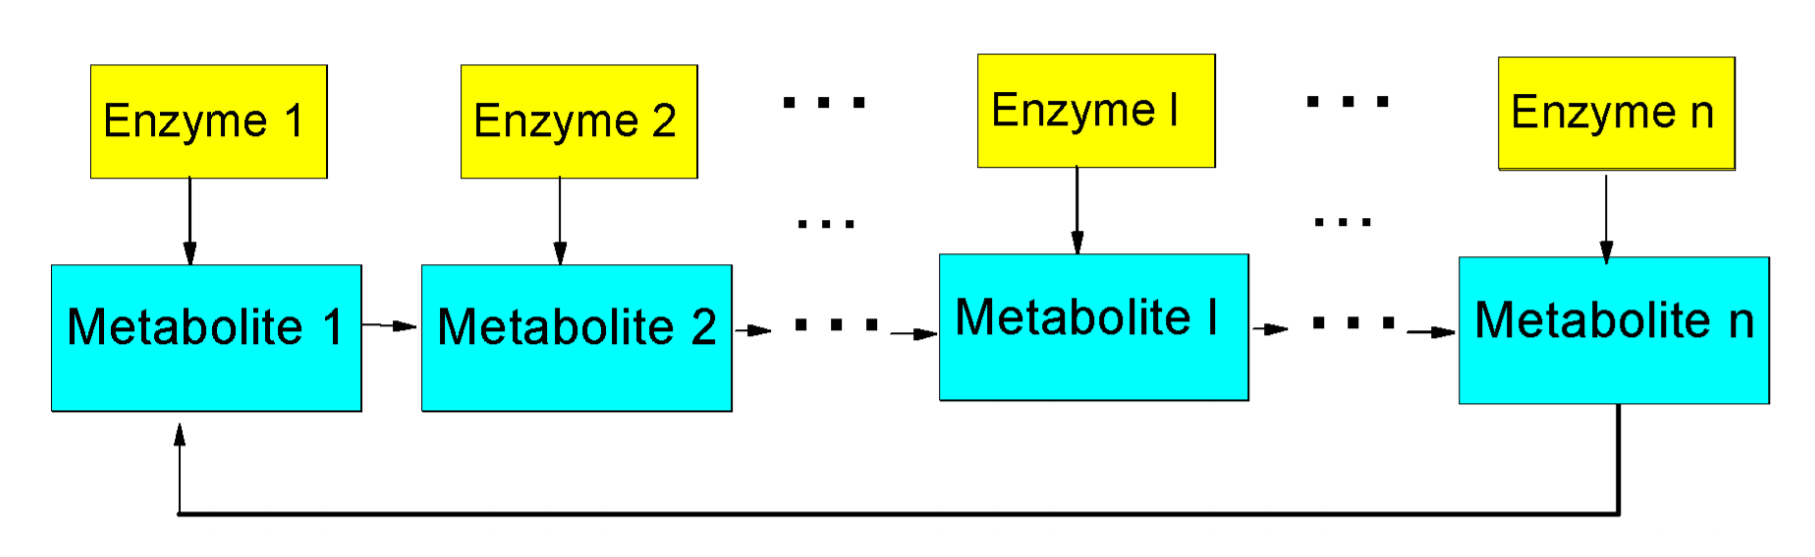
\includegraphics[scale=0.3]{img/orig-sys.png}
\end{center}

\subsection*{Rate Equations}
According to Michaelis-Menten kinetics, the rate equations 
are as given :

\begin{align*}
    \frac{d[X_i]}{dt} &= V_{\text{max}} \frac{[X_{i-1}]}{K_M + [X_{i-1}]}\\
    &= K_{i,3}[E_i]_{\text{total}} \frac{[X_{i-1}]}{\frac{K_{i,1}}{K_{i,2}} + [X_{i-1}]}\\\\
    \frac{d[E_i]}{dt} &= -K_{i,1}[E_i][X_i] + K_{i,2}[E_iX_i] + K_{i,3}[E_iX_i]\\
    &= -K_{i,1}[E_i][X_i] + (K_{i,2} + K_{i,3})\frac{[E_i]_{\text{total}}[X_i]}{K_d + [X_i]}\\\\
    \frac{d[X_iE_i]}{dt} &= k_{i,1}[X_i][E_i] - K_{i,2}[E_iX_i] + K_{i,3}[E_iX_i]\\
    &= K_{i,1}[E_i][X_i] - (K_{i,2} + K_{i,3})\frac{[E_i]_{\text{total}}[X_i]}{K_d + [X_i]}
\end{align*}

\noindent These can be further simplified, when replacing 
$[E_i]$ with $[E_i]_{\text{total}} - [X_iE_i]$. Thus the 
modified equations are :

\begin{align*}
    \frac{d[X_i]}{dt} &= K_{i,3}[E_i]_{\text{total}} \frac{[X_{i-1}]}{\frac{K_{i,1}}{K_{i,2}} + [X_{i-1}]}\\
    \frac{d[E_i]}{dt} &= -K_{i,1}[E_i]_{\text{total}}[X_i] + (K_{i,2} + K_{i,3} + [X_i])\frac{[E_i]_{\text{total}}[X_i]}{K_d + [X_i]}\\
    \frac{d[X_iE_i]}{dt} &= K_{i,1}[E_i]_{\text{total}}[X_i] - (K_{i,2} + K_{i,3} + K_{i,1}[X_i])\frac{[E_i]_{\text{total}}[X_i]}{K_d + [X_i]}
\end{align*}

\subsection*{Allosteric Binding and Negative Autoregulation}
The equations in the allosteric binding and negative 
autoregulation remain the same and thus are as follows :

\begin{align*}
    \frac{d[FP]}{dt} &= K_{rel}([FP]_{max} - [FP]) - K_{auto}[E_1]_{total}[FP]\\
    \frac{d[mRNA]}{dt} &= K_{pro}[FP] - K_d[mRNA]\\
    \frac{d[E1]_{total}}{dt} &= K_{tran}[mRNA] - K_{allo}\frac{[X_l][E_1]_{total}}{K_{half} + [E_1]_{total}}
\end{align*}

\section*{Closed Loop Systems}
Thus the rate equations for the systems are as follows :
\subsubsection*{DNA Cycle}
\begin{align*}
    \frac{d[FP]}{dt} &= K_{rel}([FP]_{max} - [FP]) - K_{auto}[E_1]_{total}[FP]\\
    \frac{d[mRNA]}{dt} &= K_{pro}[FP] - K_d[mRNA]\\
    \frac{d[E1]_{total}}{dt} &= K_{tran}[mRNA] - K_{allo}\frac{[X_l][E_1]_{total}}{K_{half} + [E_1]_{total}}
\end{align*}

\subsubsection*{Phosphorylation Cycle}

\begin{align*}
    \frac{d[X_i]}{dt} &= K_{i,3}[E_i]_{\text{total}} \frac{[X_{i-1}]}{\frac{K_{i,1}}{K_{i,2}} + [X_{i-1}]}\\
    \frac{d[X_iE_i]}{dt} &= K_{i,1}[E_i]_{\text{total}}[X_i] - (K_{i,2} + K_{i,3} + K_{i,1}[X_i])\frac{[E_i]_{\text{total}}[X_i]}{K_d + [X_i]}
\end{align*}

\subsection*{Conclusion}
Thus it can be seen that only the phosphorylation cycle has 
had any effect by changing the mechanism of calculating 
kinetics.

\section*{Analysis}
This is analysis which is done under equilibrium and various 
aspects such as robustness will be analysed.

\subsection*{Robustness}
We will use the same metric of elasticity coefficient to 
determine the robustness of the system. Thus calculation 
of $[X_l]^*$ is required which can be done by calculating 
the derivative of the latent state variable 
$[FP] + \frac{K_{rel}}{K_{pro}}[mRNA] + \frac{K_dK_{rel}}{K_{tran}K_{pro}}[E_1]_{total}$ 
which is as follows :

\begin{align*}
    &\frac{d}{dt} ([FP] + \frac{K_{rel}}{K_{pro}}[mRNA] + \frac{K_dK_{rel}}{K_{tran}K_{pro}}[E_1]_{total})\\
    =&-\frac{K_dK{rel}K_{allo}}{K_{tran}K_{pro}} \frac{[X_l][E_1]_{total}}{K_{half}+[E_1]_{total}} + K_{rel}[FP]_{max} - K_{auto}[E_1]_{total}[FP]\\
    =&-K_{gain}([X_l] - R - \frac{K_{half}[X_l]}{K_{half} + [E_1]_{total}} + \frac{K_{auto}}{K_{gain}}[E_1]_{total}[FP])
\end{align*}

It can be seen that it yields the same result and thus, from 
this, it is clear that measure of robustness will remain 
same. Thus the $[X_l]^*$ is :

\begin{align*}
    [X_l]^* &= (R - \frac{K_{auto}}{K_{gain}}[E_1]^*_{total}[FP]^*)\frac{K_{half}+[E_1]^*_{total}}{[E_1]^*_{total}}\\
    &= R(\frac{K_{rel}}{K_{auto}[E_1]^*_{total} + K_{rel}})\frac{K_{half}+[E_1]^*_{total}}{[E_1]^*_{total}}
\end{align*}

\noindent Which then leeds to the following elasticity coefficient :

\begin{equation*}
    \varepsilon = -\frac{K_{auto}[E_1]^*_{total}}{K_{auto}[E_1]^*_{total} + K_{rel}} + \frac{K_{half}}{K_{half} + [E_1]^*_{total}}
\end{equation*}

\subsection*{Conclusion}
And hence the same conclusion is drawn, which gives claim to 
the hypothesis given by the original papers' authors that it 
would remain the same.

\chapter*{Future Work}
Due to understanding and time constrains, only 
one metric was tested by me, which came out 
give the same result.
\\\\
Further work on the paper can be done, where 
even more testing is done to claims and the 
reason for the results being same can be 
tested in greater detail. 
\end{document}
